% !TEX root = ../../main.tex


\begin{figure}[!htb]
\centering
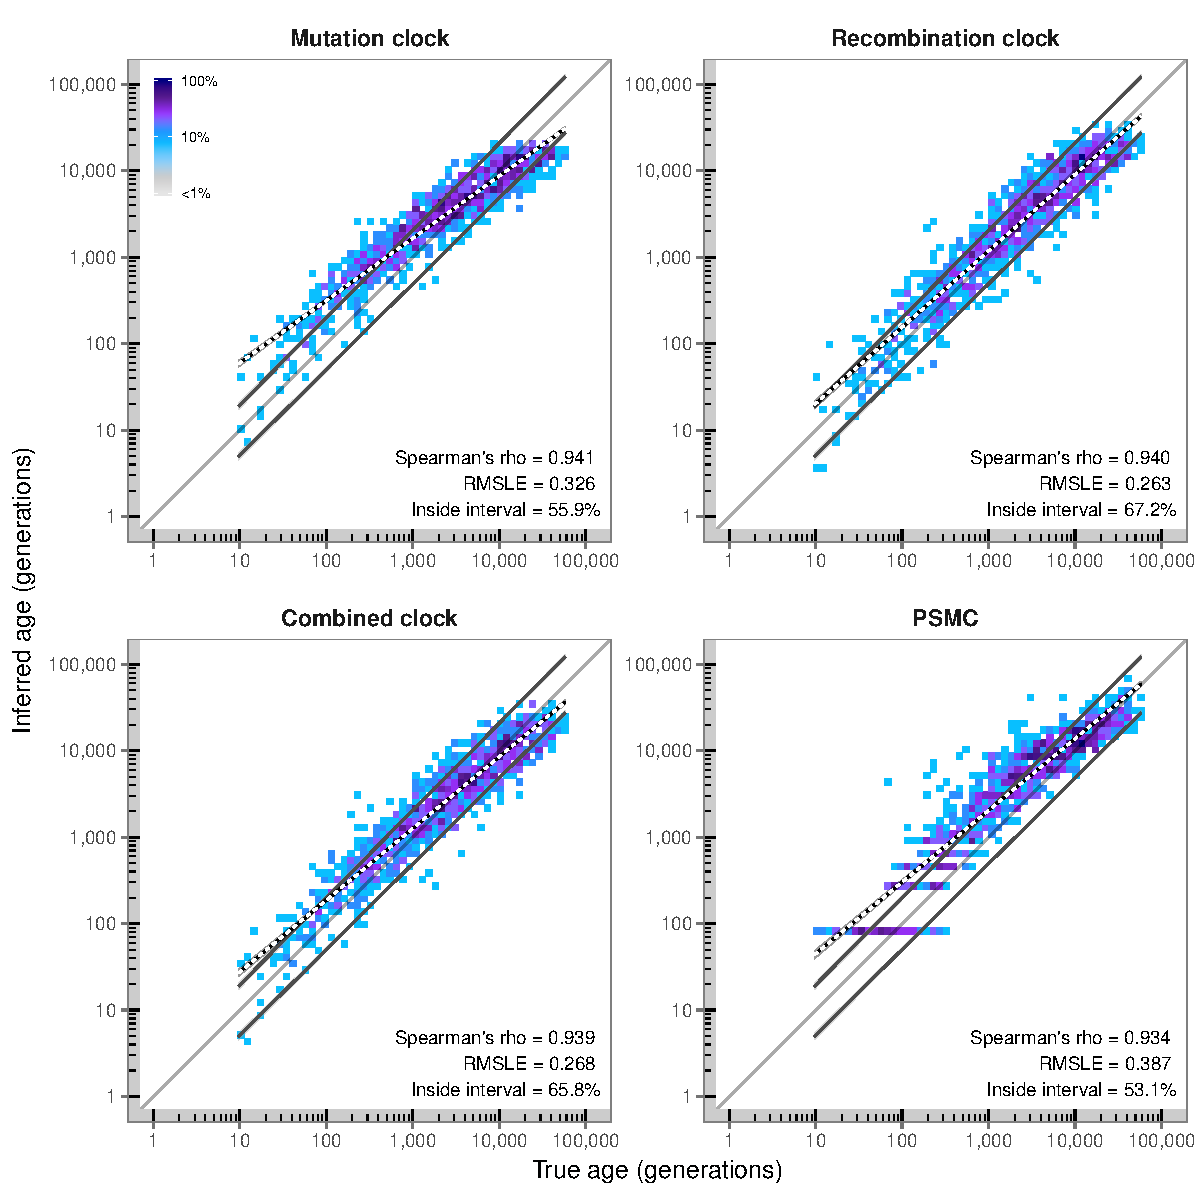
\includegraphics[width=0.9\textwidth]{./img/ch5/psmc_age}
\Caption{Allele age inferred using PSMC}%
{The \n{3} clock models (\ClockM, \ClockR, and \ClockC) were compared to \gls{psmc}.
Posterior distributions obtained on the same set of concordant and discordant pairs were used to compute the composite posterior distribution, from which point estimates were taken at the mode in each approach.
The results shown compare the ``true'' age of an allele (set at $t_m$) to the estimated age at \n{1000} target sites in dataset $\mathcal{D}_A$, which were randomly selected at allele frequency $\leq 50\%$.
Regression lines above and below the dividing line indicate the regression over $t_c$ and $t_d$.
The \emph{black-white} line shows the regression over age estimates.
Colours indicate the density of true and estimated age; scaled as the maximised density.}
{fig:psmc_age}
\end{figure}
